\setlength{\parindent}{0pt}
\chapter{\bf RESULTS}

\section{Genome-wide mapping of UV-induced damages and their repair synchronized at two stages of the cell cycle: early S phase, and late S phase}

This paper presents an experimental setup followed by bioinformatic analysis of genomic data, where we purified and sequenced fragments of \gls{uv}-induced damages and their repair in \gls{hela} cells that are synchronized either at early S phase or at late S phase. After synchronizing cells using double-thymidine treatment, we further treated cells with 20J/m\textsuperscript{2} \gls{uv}B exposure. Immediately after the exposure, we adopted Damage-seq to quantify occurred damages by the exposure, before nucleotide excision repair initiates. To quantify repair, we adopted \gls{xrseq} and quantified \gls{CPD} repair at 12 minutes and 2 hours; while \gls{64} repair were quantified only at 12 minutes (Figure \ref{fig:intro}). Finally, we performed each experiment twice to obtain biological replicates. 

Quality control analyses were performed on early S phased \gls{64}s at 12 minutes (Figure \ref{fig:intro}B-D) and other samples (Figure \ref{supfig:control1}-\ref{supfig:control8}) indicates high data qualities and consistent results between replicates. In agreement with the dual incision mechanism of nucleotide excision repair \citep{huang1992human,li2017human,reardon2005nucleotide}, \gls{xrseq} oligomers are in the size range of 20-30 nucleotides, with a median of 26 nucleotides. Moreover, dipyrimidine content of 26 nucleotides long oligomers enriches at position 19-20 (Figure \ref{fig:intro}B), where the \gls{dna} lesion occurs \citep{huang1992human}. Also, \gls{64} samples exhibit high levels of \gls{T}\gls{C} dipyrimidine repair (Figure \ref{fig:intro}B, \ref{supfig:control1}-\ref{supfig:control3}), whereas \gls{CPD} samples exhibit elevated \gls{T}\gls{T} dipyrimidine repair (Figure \ref{supfig:control4}-\ref{supfig:control8}), which are the most abundant sites for formation of these photoproducts \citep{mouret2010uva}. Because this study focuses on the \gls{gr}, contribution of \gls{tcr} can create a bias. Importantly, the repair levels at transcribed and non-transcribed strand are equivalent (Figure \ref{fig:intro}C, \ref{supfig:control1}-\ref{supfig:control8}), suggesting little or no contribution of \gls{tcr}. Correlation plots between the biological replicates indicates reasonable reproducibility, having correlation coefficients 0.86 and above (Figure \ref{fig:intro}D, \ref{supfig:control1}-\ref{supfig:control8}). 

\shorthandoff{=}
\begin{figure}[H]
    \begin{center}
    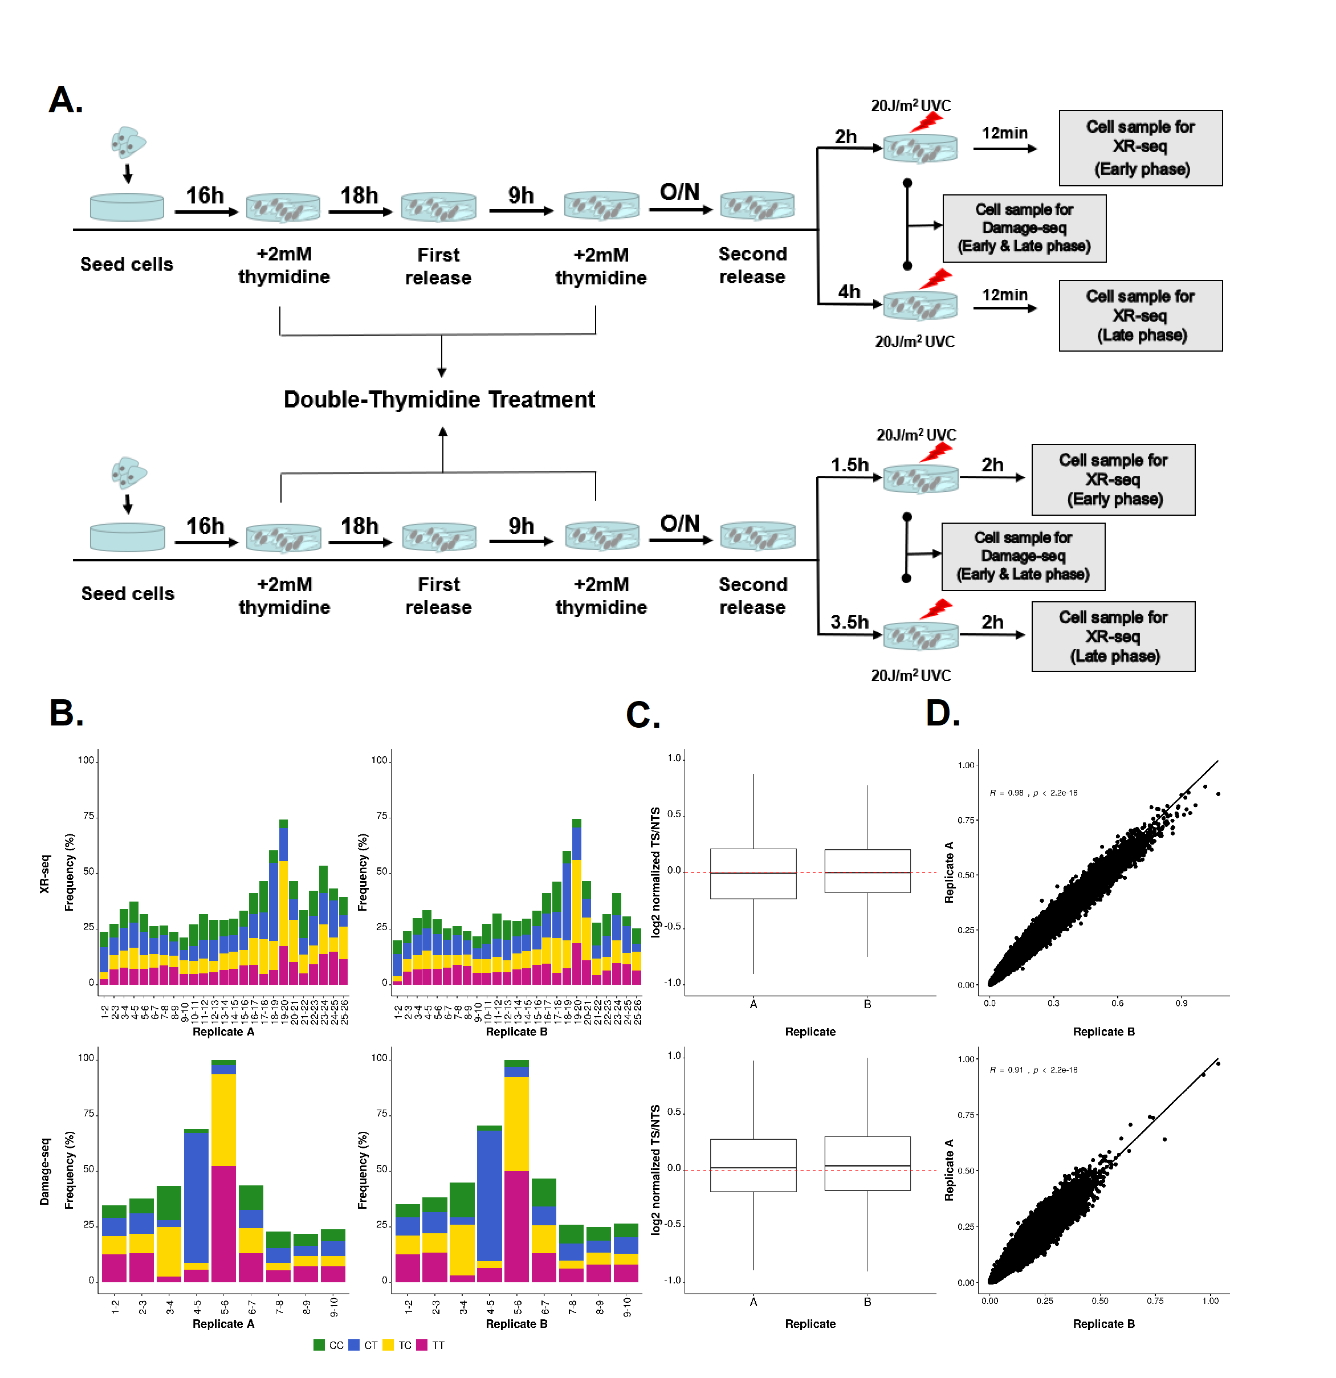
\includegraphics[width=\textwidth]{Chapters/4_results/figures/fig1}
    \caption[Experimental setup.]{A) Experimental setup. B-D) Control figures of \gls{64} early phased samples at 12 minutes. B) The dinucleotide composition frequency of replicate A and B, respectively. C) log2 transformed TS/NTS ratios of replicate A and B. Row 1 is the results of \gls{xrseq} samples, and row 2 is the results of Damage-seq samples. D) The correlation plot of the biological replicates (A \& B). Correlation coefficient is calculated by Spearman’s rank correlation test.}
    \label{fig:intro}
    \end{center}
    \end{figure}


\section{Early replication domains are repaired more efficiently than late replication domains, however, the repair rate of late replication domains elevates while replication proceeds.}

To determine how excision repair rates are influenced by replication domains during replication, we compared repair efficiency of early replication domains (\gls{erd}s) and late replication domains (\gls{lrd}s). We obtained replication domains of \gls{hela} cells from a study where a supervised method called Deep Neural Network-Hidden Markov Model was developed to define replication domains from Repli-seq data \citep{liu2016novo}. We mapped damage and repair events to corresponding replication domains. To eliminate the effect of a potential bias in damage formation, we normalized repair quantities (\gls{xrseq}) by the captured damage events (Damage-seq) in each genomic window (Figure \ref{fig:repdomain}). This approach enabled us to assess the efficiency of repair per damage at a given region, which we refer to as repair rate. Based on an analysis with a Hi-C dataset, the human genome was classified into A/B compartments, which are associated with open and closed chromatin regions, respectively \citep{lieberman2009comprehensive}. Recently, it was also shown that \gls{erd}s and \gls{lrd}s strongly correlate with A/B compartments respectively \citep{pope2014topologically,ryba2010evolutionarily}. Because \gls{erd}s are correlated to open chromatins, these regions are more reachable for excision repair machinery than \gls{lrd}s. Expectedly, repair rates of \gls{erd}s are elevated at the center and gradually reduced towards flanking sites, while \gls{lrd}s exhibit an opposite pattern (Figure \ref{fig:repdomain}A, \ref{supfig:repairrate20repdomainA}-\ref{supfig:repairrate2000repdomainB}). These results suggest that \gls{erd}s and their flanking regions are efficiently repaired, whereas less reachable \gls{lrd}s are poorly repaired. Moreover, \gls{lrd}s are known to contain higher mutation frequency than other regions \citep{lawrence2013mutational,stamatoyannopoulos2009human}, hence; low repair rate of \gls{uv} damages located at \gls{lrd}s might be a key factor of mutagenesis in melanoma cancers. 

On the other hand, the difference between early and late S phases indicates that repair rate is elevated in favor of \gls{lrd}s when replication timing moves from early to late (Figure \ref{fig:repdomain}A-B, \ref{supfig:rrel20repdomainA}-\ref{supfig:rrel2000repdomainB}). This time dependent increase in the repair rate of \gls{lrd}s can be caused by the unfolding of heterochromatin during replication. With the unfolding of the chromatin, more \gls{lrd} regions will be accessible where the \gls{dna} lesions can be recognized and removed by nucleotide excision repair. Also we observe a reduction of repair rate at \gls{erd}s, however this reduction might be caused by the relativity of the \gls{xrseq} method; increased repair rate at \gls{lrd}s results in a relative decrease in the repair rate at \gls{erd}s, even if repair rate does not quantitatively change at \gls{erd}s. In addition, \gls{64} repair at 12 minutes exhibits minor differences between early and late S phases (\ref{fig:repdomain}), potentially because of its fast repair after the damage occurrence \citep{hu2017dynamic}. Conversely, \gls{CPD} repair rate at 12 minutes and 2 hours demonstrate significant increase for \gls{lrd}s and decrease for \gls{erd}s (\ref{fig:repdomain}B, p-values < 2.2e-16). Comparison of 12 minutes to 2 hours shows that the repair rate bias is less prominent for later repair. It takes longer time to repair \gls{CPD}s relative to \gls{64}s.

\begin{figure}[H]
    \begin{center}
    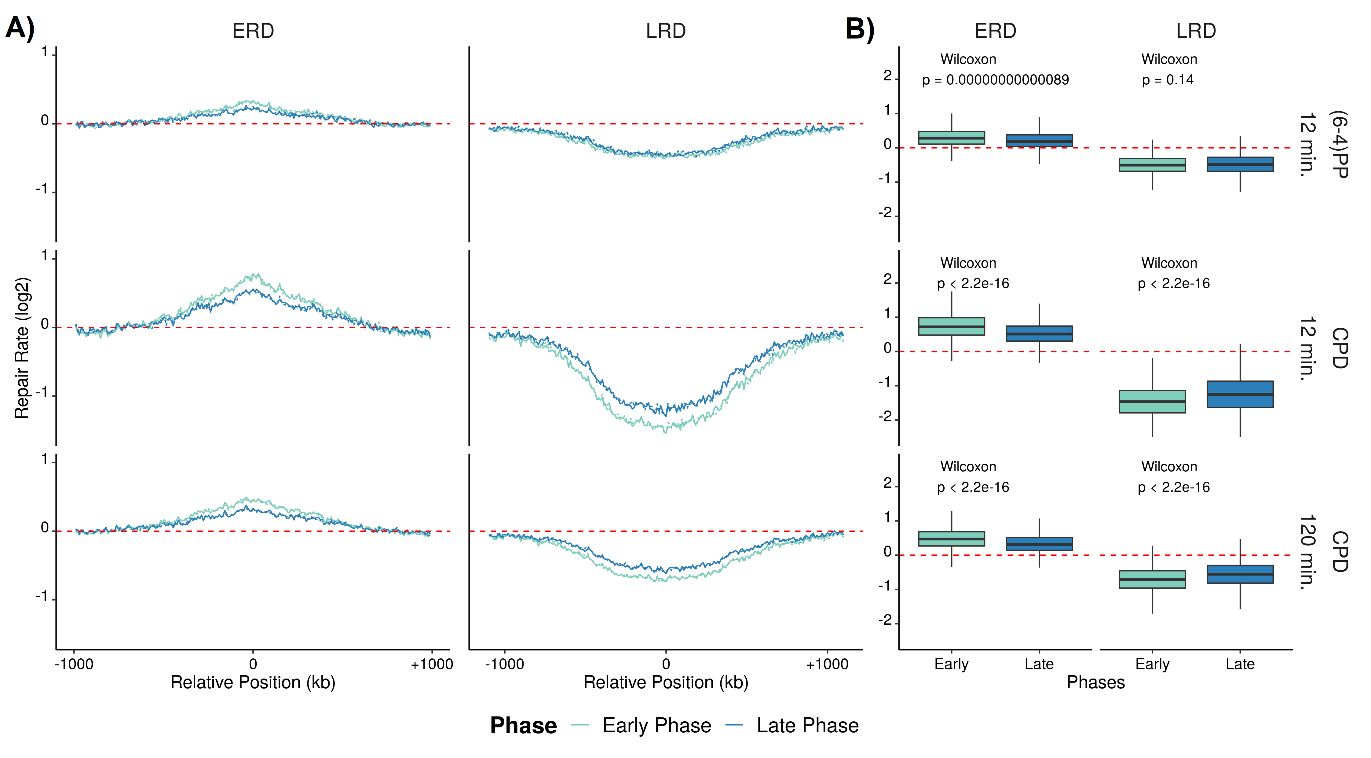
\includegraphics[width=\textwidth]{Chapters/4_results/figures/fig2}
    \caption[The shift of repair efficiency at replication domains during replication timing.]{The shift of repair efficiency at replication domains during replication timing. A) Repair rates (\gls{xrseq}/Damage-seq) are calculated and log2 transformed in 2 Mbp regions with 10 kb intervals, which early replication domains (\gls{erd}s, left) and late replication domains (\gls{lrd}s, right) positioned at the center of the region. B) \gls{rpkm} values of \gls{xrseq} samples are divided by Damage-seq samples (Repair Rate) for both \gls{erd}s (left) and \gls{lrd}s (right) and log2 transformed. Wilcoxon test is used to assess the significance of difference between early and late S phases. The light blue lines are the early phase repair rate values and dark blue lines are the late phase repair rate values. Above the red horizontal dashed line demonstrates that repair is higher than damage, below demonstrates that damage is higher. Analysis is performed on replicate A.}
    \label{fig:repdomain}
    \end{center}
    \end{figure}

\section{Variety of chromatin states are associated with dominant repair.}

Active chromatin states are repaired effectively, basically because those regions are more accessible to nucleotide excision repair \citep{adar2016genome}. We addressed how repair machinery in \gls{erd}s, and \gls{lrd}s is differentially influenced by the chromatin states during the replication. We retrieved chromatin states of \gls{hela} cells segmented by ChromHMM from \gls{ucsc} website \citep{ernst2017chromatin}. We intersected the chromatin states with replication domains and mapped damage and repair reads to those regions, for each chromosome. After calculating the repair rates (Figure \ref{fig:chromatin}A, \ref{supfig:chromatin1}A-\ref{supfig:chromatin5}A), we further assessed early S phase repair relative to late S phase (early/late repair/damage) to observe the replication timing differences in efficiency in the function of chromatin states (Figure \ref{fig:chromatin}B, \ref{supfig:chromatin1}B-\ref{supfig:chromatin5}B). Generally, repair efficiency is higher in the active chromatin states such as promoters and strong enhancers, which is in agreement with the previous studies \citep{adar2016genome, hu2016cisplatin}. Those regions sustain high repair rates, even at \gls{lrd}s during the early S phase, that should be condensed and harder to reach (Figure  \ref{fig:chromatin}A). On the other hand, all the transcription associated chromatin states together with “FaireW” and “Low” chromatin states are highly affected by the replication timing (Figure  \ref{fig:chromatin}B). “FaireW” represents the regions that are associated to the regulatory activities \citep{giresi2007faire}, whereas “Low” stands for low activity regions that neighboring active sites. On \gls{erd}s, although both chromatin states have relatively low repair at early and late S phases, they demonstrate a drastic increase when replication proceeds from early to late.  However, on \gls{lrd} regions, it is hard to make any assumptions considering the wide interquartile range of boxplots of many chromatin states (Figure  \ref{fig:chromatin}B).

\begin{figure}[H]
    \begin{center}
    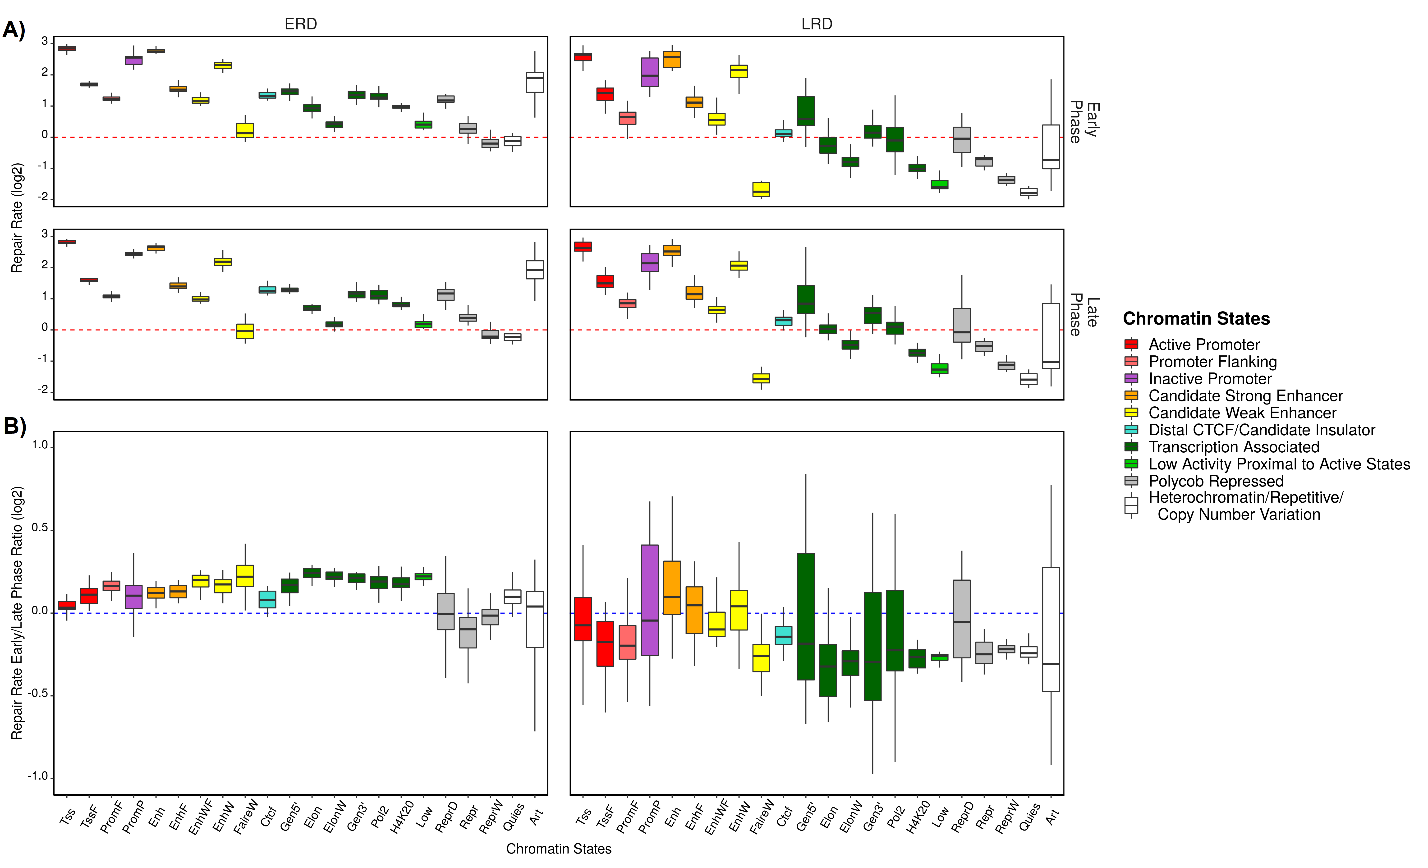
\includegraphics[width=\textwidth]{Chapters/4_results/figures/fig3}
    \caption[The effect of Chromatin States to repair efficiency of replication domains.]{The effect of Chromatin States to repair efficiency of replication domains. A) Repair rates (\gls{xrseq}/Damage-seq) of \gls{CPD} samples at 12 minutes are calculated, log2 transformed, B) and for every region, the repair rates at early S phase divided by repair rates at late S phase to spot the chromatin states that are repaired dominant at a phase. Above the red horizontal dashed line demonstrates that repair is higher than damage (A), and the blue horizontal dashed line demonstrates that the chromatin state has higher repair efficiency at early S phase than it has at late S phase (B). Analysis is performed on replicate A.}
    \label{fig:chromatin}
    \end{center}
    \end{figure}

\section{Replication origins display distinct melanoma mutation counts and strand asymmetry based on their replication domains.}

Replication domains are 1 to 2 Mb-sized \gls{dna} chunks that involves many small replication origins. Even though analyzing replication domains can exhibit the association of nucleotide excision repair and replication timing on a greater scale, the association of these small replication origins and nucleotide excision repair cannot be explained by only using replication domains. Therefore, we retrieved two independent datasets that are derived from two different methods: okazaki fragment sequencing (\gls{okseq}) and short nascent strand sequencing (\gls{snsseq}). \gls{okseq} quantifies the replication initiation zones that are the sets of closely positioned replication origins using highly purified Okazaki fragments \citep{petryk2016replication}, whereas \gls{snsseq} can precisely identifies individual replication origins \citep{besnard2012unraveling,langley2016genome}. Using these datasets together with a melanoma mutation dataset that we retrieved from the International Cancer Genome Consortium (\gls{icgc}) data portal, we examined the mutation profiles at the sites of replication origins where the replication initiates. Because nucleotide excision repair is highly associated to melanoma cancers, we argued that this relation must be reflected to the mutation counts of melanoma. For both \gls{okseq} and \gls{snsseq} data, we assorted the regions based on their corresponding replication domains to detect how mutation profiles of replication origins affected by the domains they are located. Then, we counted the mutations on these regions that are centered at individual replication origins (\gls{snsseq} data, Figure \ref{fig:mutation}A) or initiation zones (\gls{okseq} data, Figure \ref{fig:mutation}B-C) and normalized the mutations with cytosine counts in each bin, to eliminate any bias in potential mutation sites. Also, we gradually extended the region length of initiation zones from 20 kb to 200 kb (Figure \ref{fig:mutation}B-C) for observing the replication effect on a range of scales.

Mutation counts of initiation zones differ depending on the replication domains they are located. In agreement with previous studies \citep{lawrence2013mutational,schuster2012chromatin,stamatoyannopoulos2009human}, the mutation counts of initiation zones at \gls{lrd}s elevate, while \gls{erd}s contain the initiation zones with the lowest mutation counts (Figure \ref{fig:mutation}B-C). These differences that are related to the replication domains are also persistent for the individual replication origins (Figure \ref{fig:mutation}A). Furthermore, initiation zones at up (\gls{utz}s) and down transition zones (\gls{dtz}s), which are the domains that connect \gls{erd}s to \gls{lrd}s, have mutation counts in between of \gls{erd}s and \gls{lrd}s. Moreover, the flanking sites of initiation zones at transition zones that are close to \gls{erd}s have lower counts, whereas the sites that are close to \gls{lrd}s have higher (Figure \ref{fig:mutation}C, left). 
Mutation counts not only exhibit a replication domain related difference, but also reveal a strand asymmetry around the initiation zones (Figure \ref{fig:mutation}B-C). The asymmetry suggests that lagging strand (minus strand at left direction; plus strand at right direction) have more mutations than leading, independent of the replication domains. While the initiation zones at \gls{lrd}s show an explicit strand asymmetry compared to the initiation zones at \gls{erd}s, the initiation zones at \gls{erd}s have a wider strand asymmetry than that of \gls{lrd}s. One possible reason can be the amount of replication origins they harbor; earlier studies suggest that \gls{erd}s contain significantly higher number of replication origins \citep{besnard2012unraveling}, and the cumulative effect of these replication origins can create a strand asymmetry that is visible on a wider region. Additionally, replication fork movement at \gls{lrd}s (1.5–2.3 kb/min) is faster than it is at \gls{erd}s (1.1–1.2 kb/min) \citep{takebayashi2005regulation}, which can cause more mutation and increased asymmetry between strands. Conversely, individual replication origins obtained from \gls{snsseq} data do not show an explicit strand asymmetry (Figure \ref{fig:mutation}A).

\begin{figure}[H]
    \begin{center}
    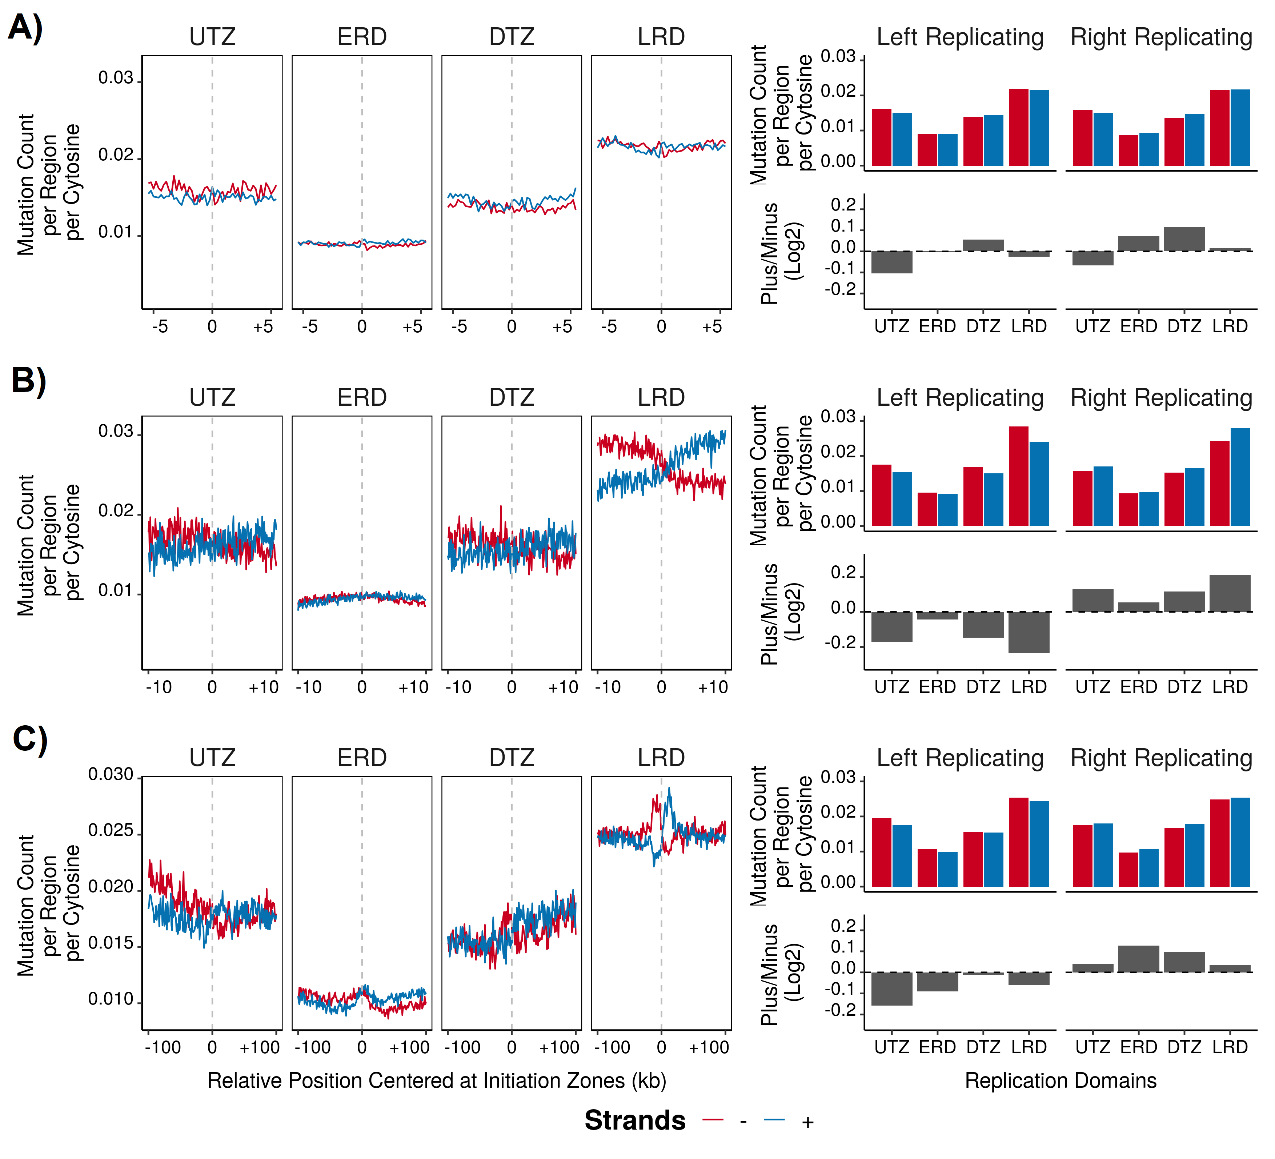
\includegraphics[width=\textwidth]{Chapters/4_results/figures/fig4}
    \caption[Tumor mutation profiles around replication origins and initiation zones for each replication domain.]{Tumor mutation profiles around replication origins and initiation zones for each replication domain. A) C to T mutations are mapped to Replication Origins (\gls{snsseq}) and counted in 10 kb regions with 100 base pair intervals. C to T mutations are mapped to Initiation Zones (\gls{okseq}) B) counted in 20 kb regions with 100 base pair intervals, C) and counted in 200 kb regions with 1000 base pair intervals. Counts are normalized by the number of regions and cytosine counts of each region. Red lines are the plus strands and blue lines are the minus strands. Gray vertical dashed line shows the center of the region. Upper right part demonstrates the strand differences at left (left part of the gray line) and right (right part of the gray line) replicating directions by taking the mean of the intervals, separately for the strands. Below that, strands are divided to each other (Plus/Minus) and log2 transformed to better visualize the asymmetry at each replication domain.}
    \label{fig:mutation}
    \end{center}
    \end{figure}

\section{Asymmetric damage around initiation zones causes asymmetric repair profiles.}

To find whether there is a strand asymmetry at repair and damage profiles similar to melanoma mutations, we mapped repair and damage events to initiation zones independently. Interestingly, A strand asymmetry around the initiation zones is visible for both repair and damage profiles (Figure \ref{fig:simulation}). The asymmetry suggests that lagging template strand harbors more damages and attracts more repair accordingly. Reasoning that nucleotide composition of initiation zones might contribute to the strand asymmetry, we decided to simulate damage and repair signals. We simulated signals via Art simulator \citep{huang2012art}, filtered the signals that resembled the real signals in nucleotide composition, and mapped the filtered ones to the human genome. The simulated signals indeed display a similar strand asymmetry, indicating the contribution of nucleotide composition of the genomic regions surrounding the initiation zones. Nonetheless, simulated signals have lower \gls{rpkm} values in general. Although nucleotide composition of these signals and real ones are similar, the real repair and damage events occurred at other regions. Therefore, it is expected to observe lower \gls{rpkm} values for simulated signals. 

\begin{figure}[H]
    \begin{center}
    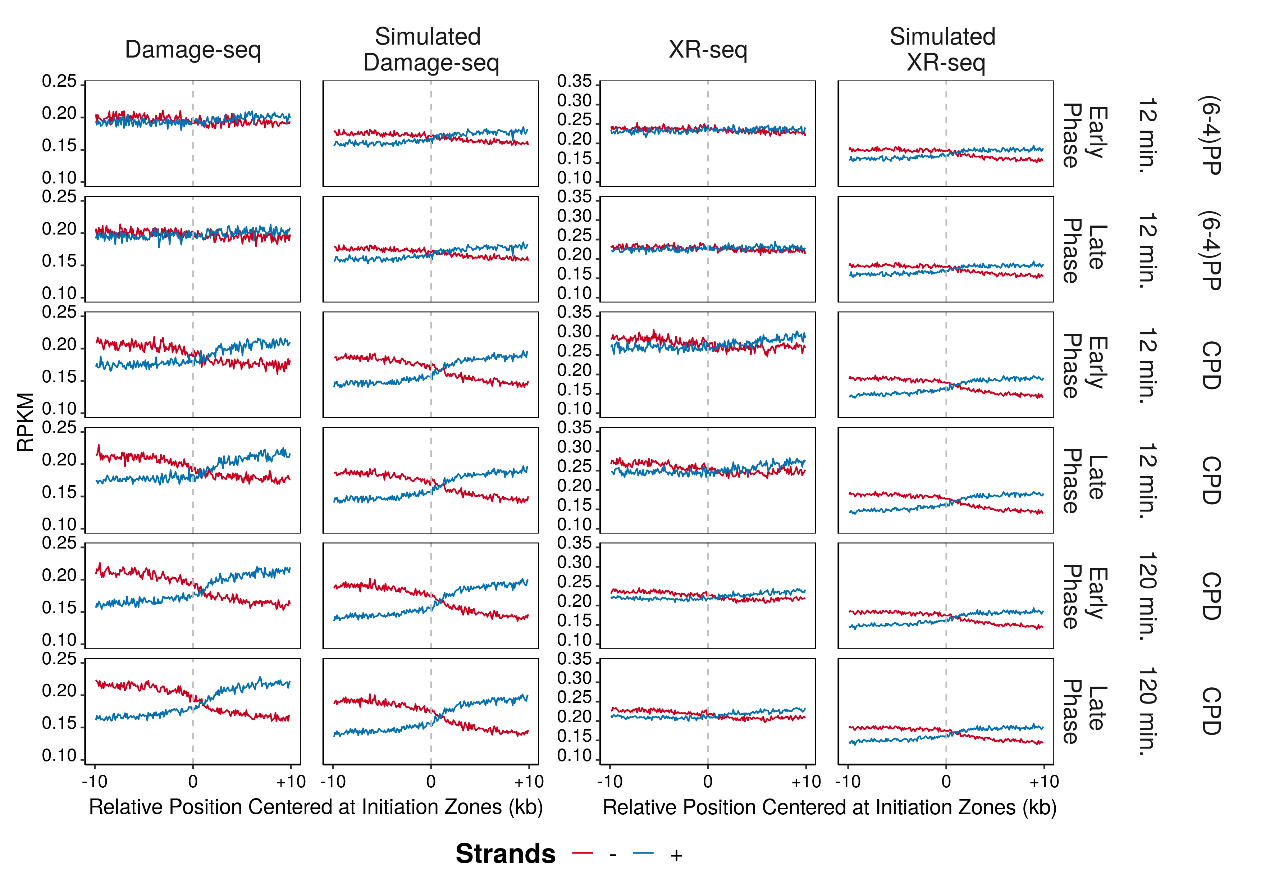
\includegraphics[width=\textwidth]{Chapters/4_results/figures/fig5}
    \caption[Strand asymmetry around initiation zones caused by sequence content.]{Strand asymmetry around initiation zones caused by sequence content. \gls{rpkm} values of real and simulated Damage-seq samples (left) and \gls{xrseq} samples (right) are calculated in 20 kb windows with 100 base pair intervals, which Initiation Zones are positioned at the center of the region. Blue lines represent the plus strands and red lines represent the minus strands. Gray vertical dashed line shows the center of the region.}
    \label{fig:simulation}
    \end{center}
    \end{figure}

\section{Strand asymmetry of excision repair rate}

After observing strand asymmetry at mutation counts of melanoma, and damage and repair events independently, we examined the repair rates of \gls{64} and \gls{CPD} samples around initiation zones for an asymmetry. Interestingly, a strand asymmetry that is inversely correlated with mutation counts of melanoma is prominent among the \gls{CPD} damages (Figure \ref{fig:repairrate}). The asymmetry indicates an efficient repair of leading strands, which is in agreement with the mutation counts that displayed low mutation on leading strands. This pattern becomes more explicit at a wider scale (Figure \ref{supfig:rr200inzonesA}, \ref{supfig:rr200inzonesB}). In addition, \gls{CPD} samples at 2 hours have elevated asymmetry at a wider scale compared to the \gls{CPD} samples at 12 minutes (Figure \ref{fig:repairrate}, \ref{supfig:rr200inzonesA}, \ref{supfig:rr200inzonesB}, \ref{supfig:rrpm20inzonesA}-\ref{supfig:rrpm200inzonesB}), because \gls{CPD}s can be effectively repaired 1 hour after the damage formation. On the contrary, samples with \gls{64} damages are not showing any strand difference, because of the fast repair ability of nucleotide excision repair for these photo-products. Although we do not observe a distinct mutational strand asymmetry at the individual replication origins, we analyzed the damage and repair events individually, and repair rates around replication origins. Surprisingly, we observed a strand asymmetry at individual replication origins (Figure \ref{supfig:rpkm10snsA}-\ref{supfig:rr20snsB}, \ref{supfig:rrpm10snsA}-\ref{supfig:rrpm20snsB}). While the samples at 2 hours demonstrates an efficient repair at leading templates, samples at 12 minutes display an asymmetry that favors the repair at lagging templates. 

Even though replication forks often move bidirectionally, at some regions, forks tend to move continuously in one direction, either by the moving long distances as a single fork, or multiple forks that are fired simultaneously \citep{takebayashi2017anatomy}. To observe the effect of replication fork movement, we decided to use the regions that replication forks move in one direction. We retrieved a data which is produced by \gls{okseq} and contains regions that are dominantly replicated in a single direction, termed high replication fork directionality (\gls{rfd}s) \citep{petryk2016replication}. Repair rates at high \gls{rfd}s display a decrease at the direction of replication fork on wider regions (Figure \ref{supfig:rr20rfdA}-\ref{supfig:rr2000rfdB}). This decrease can be caused by the replication fork itself, considering that the regions replication fork had passed opens and becomes reachable to nucleotide excision repair, while the downstream will be relatively condensed. Also, \gls{CPD}s at 2 hours demonstrate a visible strand asymmetry at both directions in favor of leading template strand (Figure \ref{supfig:rr20rfdA}-\ref{supfig:rr2000rfdB}). These results suggest that the unidirectional movement of replication fork creates a strand difference by synthesizing one strand as lagging and the opposite as leading for long regions because leading strand is repaired more efficiently.

\begin{figure}[H]
    \begin{center}
    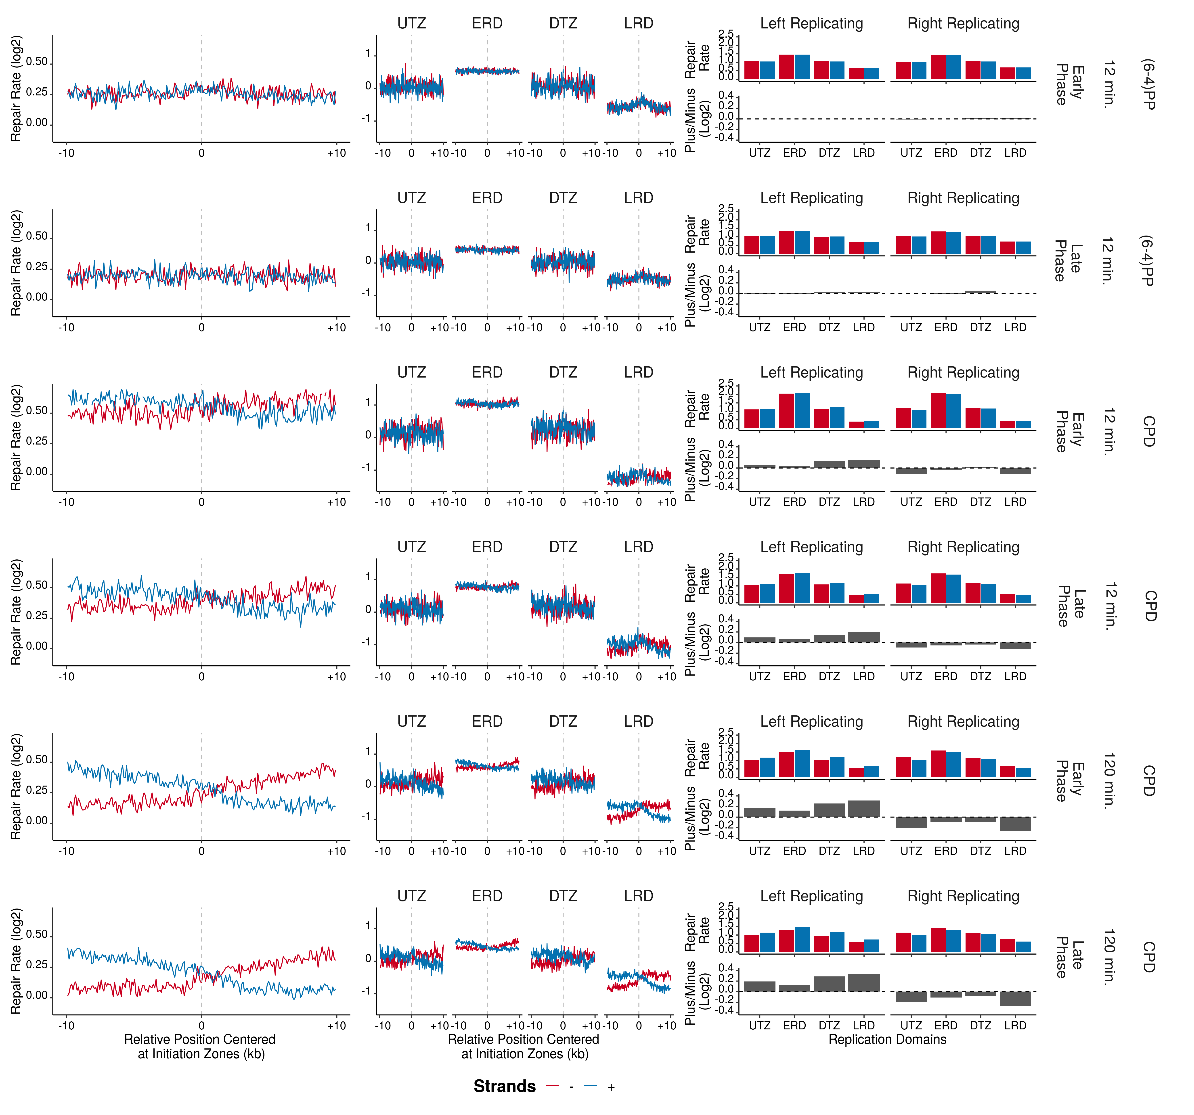
\includegraphics[width=\textwidth]{Chapters/4_results/figures/fig6}
    \caption[Repair rate asymmetry around initiation zones and replication domains.]{Repair rate asymmetry around initiation zones and replication domains. (Left) Repair rates (\gls{xrseq}/Damage-seq) are calculated and log2 transformed in 20 kb windows with 100 base pair intervals, which Initiation Zones are positioned at the center of the region. (Middle) Same analysis performed, however initiation zones separated into their corresponding replication domains. (Right) The strand differences at left (left part of the gray line) and right (right part of the gray line) replicating directions are shown by taking the mean of the intervals, separately for the strands. Below that, strands are divided to each other (Plus/Minus) and log2 transformed to better visualize the asymmetry at each replication domain. Blue lines are the plus strands and red lines are the minus strands. Gray vertical dashed line shows the center of the region.}
    \label{fig:repairrate}
    \end{center}
    \end{figure}

                                                                   
